% !TeX root = ../main.tex

\chapter{Preliminaries}

\section{Notations}
In this section, we present the notations used throughout this thesis, as listed below:

\begin{table}[H]
    \centering
    \begin{tabular}{ |p{2cm}||p{10cm}|  }
    % \begin{tabular}{ |c|l| }
        \hline
        Notation  & Definition\\
         \hline
         $\ket{0}, \ket{1}$& \\
          \hline
         $\alpha, \beta$ & The probabilies for $\ket{0}$ and $\ket{1}$\\
         \hline
         $\ket{\psi}$ & The quantum bit or qubit for short, it is used for describe linear combinations for states.\\
         \hline
         $\dagger$ & The operation that transpose and then complex conjugating the pauli matrix gate.\\
         \hline
         $\mathbb{F}_{2}$ & The finite field with two elements 0 and 1 \\
         \hline
         $\oplus$ & The XOR computation in logic representation\\
         \hline
         $E(i + j)$ & \\
    \hline
\end{tabular}
    \caption []{Some notations used in this paper}
    \label{tab:Notations}
\end{table}



\section{Quantum Circuits}
From the Enigma machine to computers based on the von Neumann architecture, all of these systems consist of wires and logic gates to execute their operations. Similarly, quantum computers are also constructed from analogous components, but instead combine quantum wires and quantum logic gates to form quantum circuits, which are used to transfer quantum bits and execute algorithms.

These are the flesh and blood of quantum computers, and we use these elements to describe the superposition state through Dirac notation:


\begin{equation}
    \ket{\psi} = \alpha\ket{0} + \beta\ket{1}
\end{equation}

In this section, we introduce some fundamental elements of quantum circuits, including the NOT, Controlled-NOT, and Toffoli gates. These gates can be understood through matrix operations, and circuits constructed using only these gates are referred to as NCT-based circuits.

Since gate-level circuits are the most commonly used construction today, we focus our efforts on reducing them.

First, the NOT gate—or, in terms of the Pauli matrices, the X gate—has an operation that can be defined by its truth table: from a classical perspective, it maps the input bit $0 \rightarrow 1$ and $1 \rightarrow 0$. From a quantum perspective, however, we can instead take the inputs as $\ket{0}$ and $\ket{1}$, and the gate acts linearly on $\ket{\psi}$. Through the matrix $X$, the state changes as follows:

\begin{figure}[h]
\centering
\begin{minipage}{0.45\textwidth}
\centering
\[
X \equiv \begin{pmatrix} 0 & 1 \\ 1 & 0 \end{pmatrix}
\]
\end{minipage}%
\hfill
\begin{minipage}{0.45\textwidth}
\centering
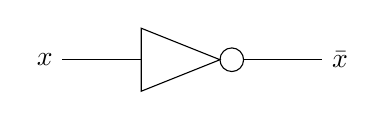
\begin{tikzpicture}
  % input wire
  \draw (0,0) -- (1,0);
  % NOT gate body (triangle)
  \draw (1,0.4) -- (1,-0.4) -- (2,0) -- cycle;
  % bubble (inversion circle)
  \draw (2.15,0) circle (0.15);
  % output wire
  \draw (2.3,0) -- (3.3,0);
  % labels
  \node[left] at (0,0) {$x$};
  \node[right] at (3.3,0) {$\bar{x}$};
\end{tikzpicture}
\end{minipage}
\end{figure}

we think about it as column view $\begin{bmatrix} \alpha \\ \beta \end{bmatrix}$

$$X\begin{bmatrix}\alpha \\ \beta\end{bmatrix} = \begin{bmatrix}\beta \\ \alpha\end{bmatrix}$$

so that it is the single qubit gates and also satisfy the \textbf{unitary} property, which means $X^{\dagger}X = I$, and it will make our input from $\alpha\ket{0} + \beta\ket{1}$ to $\alpha\ket{1}+\beta\ket{0}$ for their normalization is $|\alpha|^{2} + |\beta|^{2} = 1$.

Next, to compute the two qubit for achieve generalized XOR operation, Controlled-NOT gate or CNOT gate are most used. Exclusive-OR, what a beautiful operator, it can perfectly diffusion bit-stream in classical computer, also provide an efficient way to execution then transfer information in quantum circuit,

\section{Optimization Target}
In this work, our goal is to reduce the depth of quantum circuits as a metric, which influences both the time cost and storage cost of quantum algorithms.

Any multi-qubit logic gate can be composed from CNOT and single-qubit gates. In fact, most quantum algorithm circuits currently rely heavily on CNOT gates in gate-based quantum computers.

Therefore, shallower circuit depth can significantly decrease the number of operators required, thereby reducing the circuit's exposure to noise and quantum decoherence.

\section{Grover's Search Algorithm}